%%%%%%%%%%%%%%%%%%%%%%%%%%%%%%%%%%%%%%%%%%%%%%%%%%%%%%%%%%%%%%%%%%%%%%%%%%%%%%%%%%%%%%%%%%%%%%%%%%%%%%
%
%   Filename    : chapter_4.tex 
%
%   Description : This file will contain your Research Methodology.
%                 
%%%%%%%%%%%%%%%%%%%%%%%%%%%%%%%%%%%%%%%%%%%%%%%%%%%%%%%%%%%%%%%%%%%%%%%%%%%%%%%%%%%%%%%%%%%%%%%%%%%%%%

\chapter{Research Methodology}
% This chapter lists and discusses the specific steps and activities that will be performed by the proponent to accomplish the project. 
% The discussion covers the activities from pre-proposal to Final Thesis Writing.  It also includes an initial discussion on the theoretical
% framework to be followed.

% \section{Research Activities}
% Research activities include inquiry, survey, research, brainstorming, canvassing, consultation, review, interview, observe, experiment, design, 
% test, document, etc.  The methodology also includes the following information:

% \begin{itemize}
%   \item who is responsible for the task
%   \item the resource person to be contacted
%   \item what will be done
%   \item when and how long will the activity be done
%   \item where will it be done
%   \item why should be activity be done
% \end{itemize}

\begin{figure}[H]
    \centering
    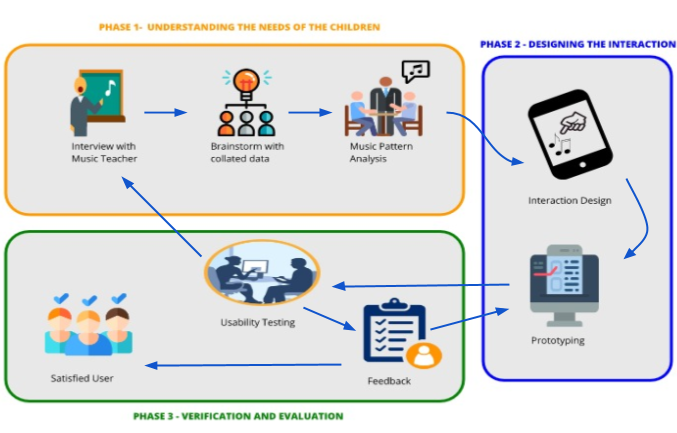
\includegraphics[width=16cm]{figures/Diagram1.png}
    \caption{Research framework for FireflyX}
    \label{fig:FireflyX}
\end{figure}

The methodology for this study can be divided into 3 phases. The first phase (see figure \ref{fig:FireflyX} Phase 1), aims to understand the students and identify their needs with the help of their music teacher. Using the data gathered from the interview with the teachers, the next phase (see figure \ref{fig:FireflyX} Phase 2) involves the designing of the interaction to solve the needs of the students. In the last phase (see figure \ref{fig:FireflyX} Phase 3) is a constant process of testing and developing on the proposed solution based on the feedback gathered in each tests.

% \section{Observation of Children Learning Music}
% Observing children while they are learning music is necessary to understand the process behind it. We will be doing this for at least 1 week in a music school for children aged 7-9 in the span of an hour. We will be using their classroom where they usually hold their music classes to conduct the observation. The activity will be recorded with a camera and a voice recorder for backup in case the camera fails. All members will take notes on a notebook of the interactions of the students and the teacher. By doing these, we can also ensure that we can properly optimize and cater our app for children learning. The main goal of this activity is to find points that we can improve on and find problems or difficulties that children are experiencing.

\section{Interview with the Music Teacher}
An interview with the music teacher of the children was done in order to understand the process of how children are taught music. The interview served as confirmation for the observations we made in the previous activity. This interview will also expand our knowledge on music and identify aspects that might not have been covered by previous observations. The interview was conducted in a secluded room where only the interviewer and the interviewee are present in order to minimize distractions in addition to this, a backup voice recorded. Observations was also written down on a notebook. The notes taken during the interview was used for discussion within the group to collate and brainstorm.

The main questions asked in the interviews are:
\begin{enumerate}
    % \item What are your thoughts on children and music?
    % \item Have you taught or are teaching anyone music?
    % \item Have you taught or are teaching children?
    %     If yes to both,
	   %     Have you taught or are teaching music to children?
    % \item What music concepts do you usually teach children ages of 5-8?
    % \item How would you teach these concepts to these children?
    % \item Do you think that the children are learning these concepts?
    % \item Is it difficult to teach music?
    % \item What about for teaching music to children?
    % \item What makes it different when teaching children?
    % \item What difficulties do children usually encounter when learning music?
    % \item What techniques or methods did you use to overcome these difficulties?
    % \item How do you suggest children should learn music?
    % \item What are signs that a child is learning a music concept?
    % \item Do you conduct tests?
    % \item If yes, what kind of tests do you conduct? If no, how do you evaluate if a child is learning music?
    % \item Do you have any suggestions on how to interact with children?
    \item How long have you been teaching music?
    \item Have you thought or are teaching children?
    \item How do you start your sessions with children?
    \item Do you have special techniques when teaching children?
    \item Do you use the same techniques with all the children?
    \item What difficulties do you encounter when you teach children?
    \item Do you keep in contact with the student outside the classroom?
    \item What role do the parents have in the learning journey of the child?
\end{enumerate}

The questions above are non-exhaustive and may lead to more follow up questions. Different questions may be inserted or added depending on how the musician would answer a question to gather more data or insights.

\section{Brainstorming on Collated Data}
After the observation and interview, it is necessary that we analyze and process the data acquired through a meeting. All data gathered was stored on a Google Drive and a flash drive for backup in case of lost files. Based on the problem statement, we then developed ideas and shared these ideas among ourselves. The group then tried to synthesize and improve on each idea. A scenario map was made based on how the teachers perceive the learning experience of children. The scenario map highlights the process of the children using the app. Personas were also made in order to identify which helps us identify the specific needs of the personas and better suit the prototype and app in order to cater the personas. The resulting list of features and solutions would then be consulted to a music expert to determine if a prototype will be possible or usable for children.

% \section{Consulting with Music Expert}
% % An interview with a music expert will be done in order to understand the process of how children understand music. The interview will also help us validate and confirm the observations we made in the previous activity. This interview will also expand our knowledge on music theories and also to identify aspects that might not have been covered by previous observations. Like the interview with the music teacher, the interview will be conducted in a secluded room, recorded by camera and voice. Observations will also be taken note of and finally the notes taken during the interview will be used for discussion within the group to collate and brainstorm.
% Once the team has finished brainstorming on potential solutions, we would set an interview with the music expert. This is done as we would want to verify what the teacher said to us during the interview and how the children acted during our observation of them. Also we would want to know if the data gathered is true based on musical theory. For the consideration of our music expert we would want him/her to have many experiences on the field of music and also children. 

The main questions asked in the consultation are:
\begin{enumerate}
    \item Have you taught music to children of age 5-8?
    \item What are the musical theories that children of age 5-8 should be learning?
    \item What are some of the difficulties in teaching music to children?
    \item How did you overcome these difficulties?
    \item Do you have any suggestions on how to interact with children?
    \item How did you assess the learning of the children?
    \item Were the observations we made on the children accurate?
    \item What areas are important to observe when conducting activities with children?
    \item Was the assessment of the teacher based on our observation of the children accurate?
    \item What are some suggestions you can give on how we should design our system based on our observations?
    \item Do you have any suggestions on what features would be important for the app?
\end{enumerate}

The questions above are non-exhaustive and may lead to more follow up questions. Different questions may be inserted or added depending on how the musician would answer a question to gather more data or insights.

\section{Music Pattern Analysis}
Rhythmic music patterns acquired from the Suzuki Book 1 will be analyzed. The most frequent clap-reset combination was taken into account and included in the Library of Patterns (Refer to Table \ref{Patterns}). We also looked at music sheets for piano to help us in modeling patterns found with the integration of different pitches. We took inspiration from the idea of Nyquist to make these patterns and represent them in Swift. This also gave us an idea on which claps and notes would be used for the mapping of the firefly model. Included in this would be the amount of claps per measure, measures per section, and the amount of sections per rhythm. All of these will be considered when deciding on the possible firefly configurations.

\section{Interaction Design and Prototyping}
Using the input given by the teacher and music expert, concepts for the initial interaction design are to be sketched out on paper. The sketches will be based on how the mapping of the firefly model will be, and from the features developed from the previous activities. The sketches will also be tested first by the teacher before being implemented into a mockup. Feedbacks and suggestions will also be gathered to improve the sketches and mockups. Multiple designs are to be created based on how each member's ideas on how to solve the problems of the students. 

Once a design was agreed upon by each member of the group, a mid-fidelity prototype is to be made using Figma to design for the proposed interface of the app based on the observation, interview, and consultations done in the previous activities. The decisions for the mappings of the firefly will also be decided in this part. The music patterns analyzed from the activity before will be used here to decide which features from the music patterns will be mapped to a firefly part. Music fundamentals like rhythm, tempo and pitch will also be mapped to a specific firefly part.

Like the activities before, feedback will be gathered in order to improve the prototype. Even though there will be limited functionality and features in the prototype, this will give us a better idea before developing the actual app.

\section{Implementing and Testing the Prototypes}
An agile software development methodology will be implemented. The software engineering approach will be iterative, where we will take into account the feedback and suggestions of the users to improve the next iteration. A GitHub repository will be created to store and to have save points for the prototype. The prototype will be updated every time after we analyze and collate the data. Updates will be pushed to a GitHub repository when we have decided on a proper update. The GitHub repository will also serve as an access point for the members of the group. 

After developing the app, usability tests will be performed with the objective of determining the overall experience in using the app. Before starting the test, the testers will first be given a consent form along as the consent from their parents. If they agree with the terms and decided to continue with the testing, they will be given a brief introduction and description of the study along with the objectives and overview. They will then be asked to use Firefly and be assessed after. During the test we will encourage the child to think aloud as this will help us in gathering more inputs on the human factors they exhibit in doing the tasks. For the test setup these will be conducted where there is little to no audio and visual distractions. This will ensure that the users will be focused, and also to maintain the clear audio and video while recording. The latest version of firefly installed in a tablet iPad will be provided to the tester of the application. There will be two cameras recording the tester, the first is the camera of the laptop that records the facial expressions. This will be needed to see the reactions of the tester. The second camera records the gestures with the interaction with the application. The tasks will be written on a piece of paper that is visible for the child to see in the table. These will all be recorded using an audio recording device to capture the audio to be used for the transcription of the user testing. 

The evaluation for the test will be digital and will be operated by the test moderator. The test moderator will ask the child questions and will then record the answers of the child in the form. The quantitative data will also be acquired in the evaluation mentioned earlier. This form of data is to be used in evaluating the usability data of the applications different features. This is done by the group to identify the features that have caused inconveniences for the users. The data will then be analyzed to improve the app and factor in the feedback acquired from the testing. Sample questions will be written in the different iterations of testing below. Interviews will also be done after the testing to validate the observations and also to get feedback on the user experience of the children testing the application. The adult companion and the teacher will be able to accompany and watch the child during testing.

For the first and second iteration it will be following the diagram shown in figure \ref{test1and2}.

\begin{figure}[H]
    \centering
    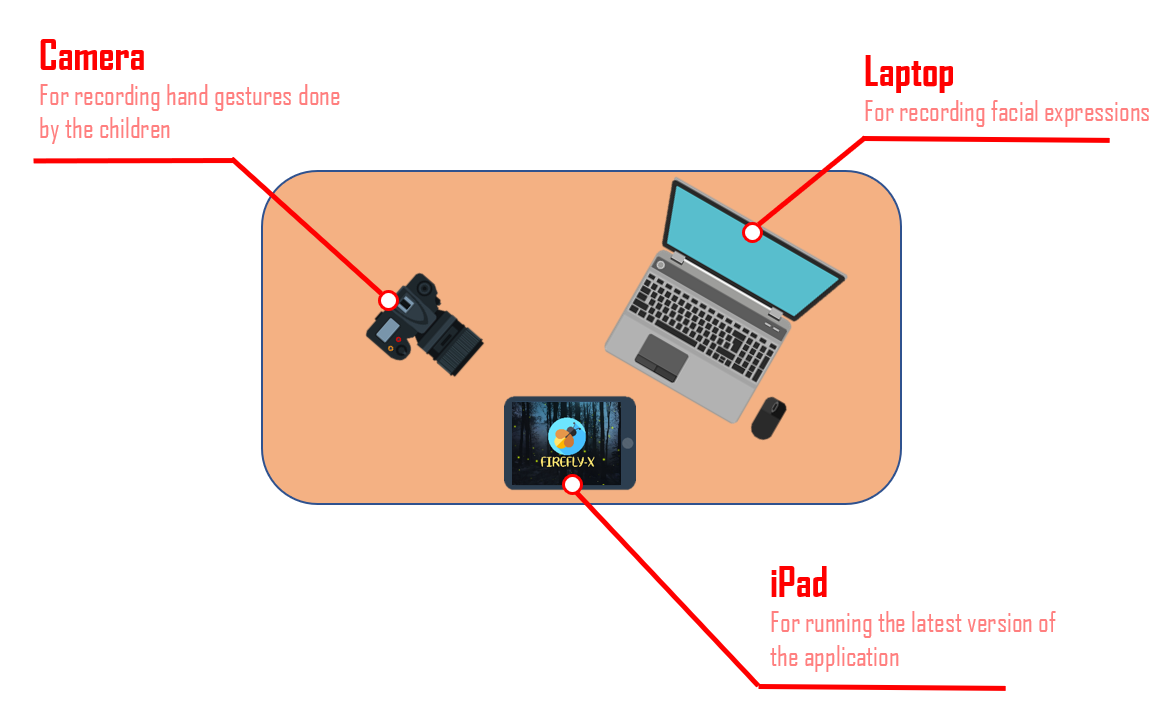
\includegraphics[width=15cm]{figures/Test_Setup.png}
    \caption{Iteration 1 and 2 Test Setup}
    \label{test1and2}
\end{figure}

The testers, music students aged 5-8 from different music schools will be asked to take part in the data collection and testing. Testing will be divided into three (3) phases with each iteration having a set of different tasks since more features are to be added in the application per iteration. 

Tasks that will be asked to do will be modeled from the use cases found in Appendix \ref{sec:appendixc}.

\subsection{First Iteration}
After developing the application which is 60\% complete, it would be tested with three (3) users. Since the functionality at this iteration is still at 60\%, we would like the users to test mainly on the fundamental functionality with only one firefly. These tasks revolve around the manipulation of the parts/functionality of the firefly. To meet 60\% completeness namely the tail (pattern), wing (repetition), body (tempo), wing (note speed), and the playback engine. 

These are examples of tasks that will be asked to be done for the first iteration:
\begin{itemize}
    \item Set the tempo of the firefly by choosing a body type
    \item Set the number of repetitions of the firefly by choosing a setting in the right wing
    \item Set the speed of note of the firefly by choosing a setting in the left wing
    \item Set the blinking pattern of the firefly by choosing a tail type
    \item Replace the tempo by selecting a different body type
    \item Replace the current repetition by selecting a different setting in the left wing
    \item Replace the current speed of note by selecting a different setting in the right wing
    \item Replace the pattern by selecting a different tail type
    \item Tap start to start playing the firefly
    \item Tap stop to stop the firefly from playing
    \item Tap on the power button to exit to main menu
\end{itemize}

These are the sample questions in the evaluation with the scale being 1 being the easiest to 5 being difficult. We will be asking these to tester to better understand the functionality of the first iteration:

\begin{itemize}
    \item How difficult was it to set the tempo? 
    \item How difficult was it to set the repetition? 
    \item How difficult was it to set the speed of the note? 
    \item How difficult was it to set the clap-rest pattern? 
    \item How difficult was it to replace the current tempo? 
    \item How difficult was it to replace the current repetition? 
    \item How difficult was it to replace the current speed of the note? 
    \item How difficult was it to replace the current clap-rest pattern? 
    \item How difficult was it to start playing the firefly?
    \item How difficult was it to stop to stop the firefly from playing?
    \item Was it difficult to go through the application?
    \item Do you like the design of the application?
    \item Was the functionality of the parts clearly seen?
\end{itemize}

\subsection{Second Iteration}
In the second iteration we would then test the application that is 80\% complete with seven (7) testers. From the seven testers three of them will be retained from the first iteration of testing, meaning we would have four new participants for this iteration. In this iteration we will be implementing the changes based on the comments received from the first iteration of testing. The aim is to be 80\% wherein there will still be one firefly playing. Functionalities such as pitch and release to canvas, in addition with the ability to manipulate the firefly parts will be added to meet the 80\% completeness.

The tasks from the first iteration will carry on in the second iteration testing. These are examples of newly added tasks that will be asked to be done for the second iteration:
\begin{itemize}
    \item Tap pause to pause the firefly from playing 
    \item Tap resume to resume the playing of the firefly
    \item Tap the jar to replay previous fireflies 
    \item Tap on the Feed Me Button to start changing the pitch
    \item Set the pitch of each note by dragging the biscuit on the tray to the staff
    \item Start replacing the current pitch of a note by clicking Feed Me button again
    \item Replace the current pitch for one or more notes by dragging the biscuit/s to a higher line in the staff
    \item Replace the current pitch for one or more notes by dragging the biscuit/s to a lower line in the staff
    \item Clear the pitch for all notes by selecting the Clear button 
    \item Preview the pitch representation of the firefly by selecting the Preview button 
\end{itemize}

These are the sample questions in the evaluation with the scale being 1 being the easiest to 5 being difficult. Aside from the questions that we will ask again that came from iteration 1 we will be introducing these new questions to the tester to better understand the functionality of the second iteration:

\begin{itemize}
    \item How difficult was it to pause the firefly from playing?
    \item How difficult was it to resume the playing of the firefly?
    \item How difficult was it to to replay previous fireflies?
    \item How difficult was it to set the pitch? 
    \item How difficult was it to replace the current pitch to a higher position in the staff? 
    \item How difficult was it to replace the current pitch to a lower position in the staff?
    \item How difficult was it to clear all pitches? 
    \item How difficult was it to preview the pitch playback? 
\end{itemize}

\subsection{Third Iteration}
Lastly in the third iteration, fifteen (15) users will be testing the complete application. Where same as the second iteration we will retain the seven users that already have tested the application previously and we will get eight new participants in this last iteration. The last stage revolves on improving the functionality from the first two stages. Functionality in this stage for it to be fully complete should already handle five (5) fireflies as well as saving and loading the workspace. The tasks will also use the same as the first two iterations and also adding the new functionality developed in this last iteration. For the last iteration since new tasks on composing will be added we will be also adding a music sheet in the test setup as seen in figure \ref{test3}.

\begin{figure}[H]
    \centering
    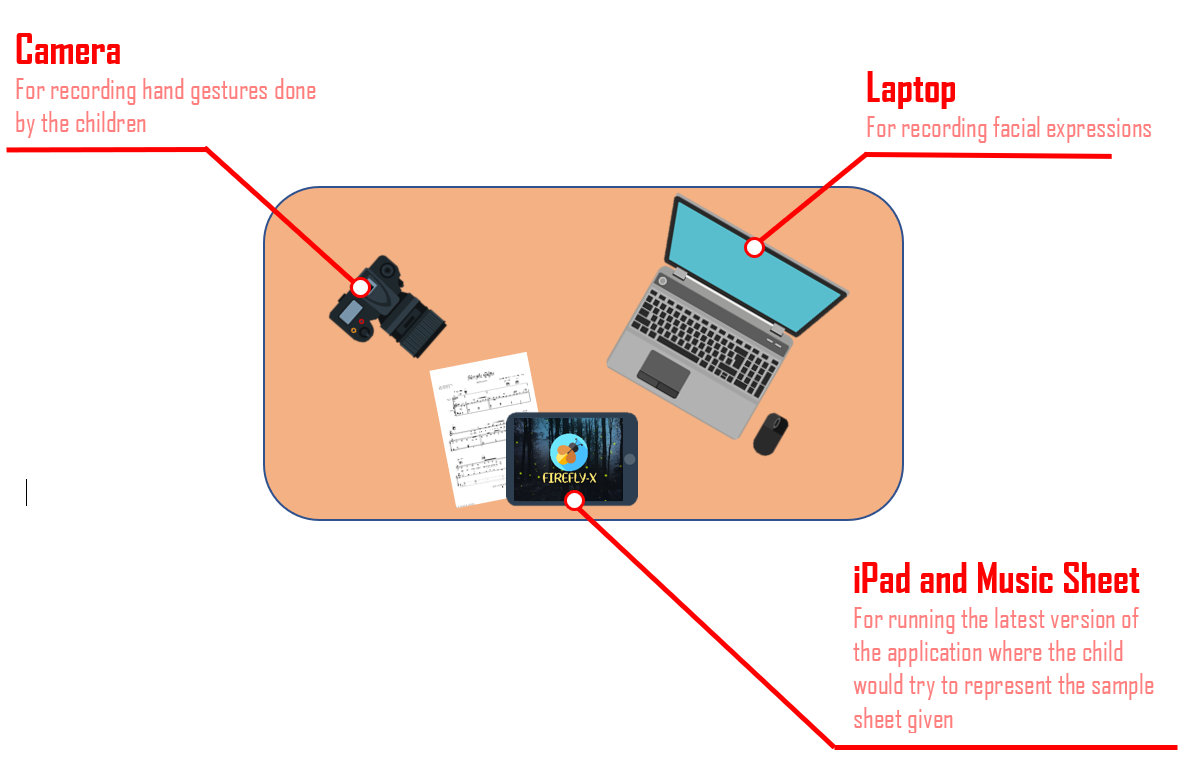
\includegraphics[width=15cm]{figures/Test_Setup_Last.png}
    \caption{Iteration 3 Test Setup}
    \label{test3}
\end{figure}

The tasks from the first and second iteration will carry on in the third iteration testing. These are examples of newly added tasks that will be asked to be done for the third iteration:
\begin{itemize}
    \item Tap Reset Album to reset the fireflies
    \item Tap Save to save the modified fireflies
    \item Tap Load to load previously made fireflies
    \item Configure the fireflies to emulate a sample sheet given by the testers (Hot Cross Buns)
    \item Configure the fireflies to make a simple familiar song like (Twinkle Twinkle Little Star/Happy Birthday)
    \item Edit the fireflies to modify a previously made track
    \item Free play of the environment
    \item Configure five fireflies
\end{itemize}

These are the sample questions in the evaluation with the scale being 1 being the easiest to 5 being difficult. Aside from the questions that we will ask again that came from iteration 1 we will be introducing these new questions to the tester to better understand the functionality of the second iteration:

\begin{itemize}
    \item How difficult was it to to reset the fireflies?
    \item How difficult was it to save the modified fireflies?
    \item How difficult was it to load previously made fireflies?
    \item How difficult was it to copy the sample sheet Hot Cross Buns using the fireflies? 
    \item How difficult was it to modify a previously made track? 
    \item How difficult was it to freely play the application?
    \item How difficult was it to configure the five fireflies in an environment?
    \item How would you rate the learning you got from the application?
\end{itemize}

% Sample questions asked in different iterations of feedback from the users:
% \begin{enumerate}
%     \item How much did you use this feature to accomplish the tasks?
%     \item On a scale of 1 to 4 (with 4 being the highest and 1 being the lowest) were you comfortable while using this feature?
%     \item Is there any need to improve this feature? Why?
% \end{enumerate}

% \section{Usability Testing}

% \section{Feedback}
% The feedback from testing will come in forms of qualitative and quantitative data. Qualitative data will be acquired through video recordings, observations, and interviews. The setup will include cameras to capture the facial expressions and hand gestures while the children are testing the application. Interviews will also be done after the testing to validate the observations and also to get feedback on the user experience of the children testing the application. The quantitative data will also be acquired in forms of a questionnaire. This form of data is to be used in evaluating the usability data of the applications different features. This is done for the group to identify the features that have caused inconveniences for the users. A scale from 1-4 will be asked from the testers with the assistance of the teacher with 4 being the highest and 1 being the lowest. 



\begin{landscape}
\section{Gantt Chart}
% \begin{table}[H]
% \centering
% \caption{Timetable of Activities} \vspace{0.25em}
% \begin{tabular}{|l|l|l|l|l|l|l|l|l|l|l|l|l|l|l|l|l|}
%     \hline
%     2019 - 2020                  & May  & Jun   & July & Aug  & Sep & Oct & Nov & Dec & Jan  & Feb  & Mar  & Apr & May  & Jun  & Jul  & Aug \\ \hline
%     Planning                     & \textbullet    & \textbullet     & \textbullet    & \textbullet    & ~   & ~   & ~   & ~   & ~    & ~    & ~    & ~   & ~    & ~    & ~    & ~   \\ \hline
%     RRL & \textbullet\textbullet\textbullet\textbullet & \textbullet\textbullet\textbullet\textbullet & \textbullet\textbullet\textbullet\textbullet & \textbullet\textbullet\textbullet\textbullet & ~   & ~   & ~   & ~   & ~    & ~    & ~    & ~   & ~    & ~    & ~    & ~   \\ \hline
%     Learning Swift      & ~    & ~     & \textbullet\textbullet\textbullet & \textbullet\textbullet\textbullet  & \textbullet\textbullet  & \textbullet   & \textbullet   & ~   & ~    & ~    & ~    & ~   & ~    & ~    & ~    & ~   \\ \hline
%     Development                  & ~    & ~     & ~    & ~    & ~   & \textbullet\textbullet\textbullet\textbullet   & \textbullet\textbullet\textbullet\textbullet   & \textbullet\textbullet\textbullet  & \textbullet\textbullet\textbullet\textbullet & \textbullet\textbullet\textbullet\textbullet & \textbullet\textbullet\textbullet\textbullet & \textbullet\textbullet  & ~    & ~    & ~    & ~   \\ \hline
%     Experiment Design              & ~    & ~     & ~    & ~    & ~   & ~   & ~   & ~   & ~    & \textbullet    & \textbullet\textbullet   & \textbullet\textbullet  & ~    & ~    & ~    & ~   \\ \hline
%     Results and Analysis         & ~    & ~     & ~    & ~    & \textbullet \textbullet   & \textbullet \textbullet \textbullet \textbullet   & \textbullet   & ~   & ~    & ~    & ~    & \textbullet\textbullet\textbullet & \textbullet\textbullet\textbullet\textbullet & \textbullet\textbullet\textbullet\textbullet & ~    & ~   \\ \hline
%     Documentation                & \textbullet    & \textbullet     & \textbullet    & \textbullet    & \textbullet   & \textbullet   & \textbullet   & \textbullet   & \textbullet    & \textbullet    & \textbullet    & \textbullet   & \textbullet\textbullet   & \textbullet\textbullet\textbullet\textbullet & \textbullet\textbullet\textbullet\textbullet & \textbullet   \\ \hline
% \end{tabular}
% \label{tab:ganttChart}
% \end{table}
% Please add the following required packages to your document preamble:
% \usepackage[normalem]{ulem}
% \useunder{\uline}{\ul}{}
\begin{table}[H]
\caption{Timetable of Activities} \vspace{0.25em}
\label{tab:ganttChart}
\begin{tabular}{|l|l|l|l|l|l|l|l|l|l|l|l|l|l|l|l|l|}
\hline
2019 - 2020                                                                & May                                                                                                      & Jun                                                                                                      & July                                                                                                     & Aug                                                                                                      & Sep                                                                                                      & Oct                                                                                                         & Nov                                                                                                      & Dec                                                                            & Jan                                                                                                      & Feb                                                                                                      & Mar                                                                                                      & Apr                                                                            & May                                                                                                      & Jun                                                                                                      & Jul                                                                                                      & Aug                        \\ \hline
Planning                                                                   & \textbullet                                                                               & \textbullet                                                                               & \textbullet                                                                               & \textbullet                                                                               &                                                                                                          &                                                                                                             &                                                                                                          &                                                                                &                                                                                                          &                                                                                                          &                                                                                                          &                                                                                &                                                                                                          &                                                                                                          &                                                                                                          &                            \\ \hline
RRL                                                                        & \textbullet\textbullet\textbullet\textbullet & \textbullet\textbullet\textbullet\textbullet & \textbullet\textbullet\textbullet\textbullet & \textbullet\textbullet\textbullet\textbullet &                                                                                                          &                                                                                                             &                                                                                                          &                                                                                &                                                                                                          &                                                                                                          &                                                                                                          &                                                                                &                                                                                                          &                                                                                                          &                                                                                                          &                            \\ \hline
Interview                                                                  &                                                                                                          &                                                                                                          &                                                                                                          &                                                                                                          & \textbullet\textbullet\textbullet\textbullet & \textbullet                                                                                  &                                                                                                          &                                                                                &                                                                                                          &                                                                                                          &                                                                                                          &                                                                                &                                                                                                          &                                                                                                          &                                                                                                          &                            \\ \hline
\begin{tabular}[c]{@{}l@{}}Preliminary Results\\ and Analysis\end{tabular} &                                                                                                          &                                                                                                          &                                                                                                          &                                                                                                          &                                                                                                          & \textbullet\textbullet\textbullet\textbullet    &                                                                                                          &                                                                                &                                                                                                          &                                                                                                          &                                                                                                          &                                                                                &                                                                                                          &                                                                                                          &                                                                                                          &                            \\ \hline
Learning Swift                                                             &                                                                                                          &                                                                                                          &                                                                                                          &                                                                                                          &                                                                                                          &                                                                                                             & \textbullet\textbullet\textbullet\textbullet                                                                               &  \textbullet\textbullet                                                                             &      \textbullet\textbullet\textbullet\textbullet                                                                                                    &                                                                                                          &                                                                                                          &                                                                                &                                                                                                          &                                                                                                          &                                                                                                          &                            \\ \hline
Development                                                                &                                                                                                          &                                                                                                          &                                                                                                          &                                                                                                          &                                                                                                          & \textbullet\textbullet\textbullet\textbullet    & \textbullet\textbullet\textbullet\textbullet & \textbullet\textbullet\textbullet & \textbullet\textbullet\textbullet\textbullet & \textbullet\textbullet\textbullet\textbullet & \textbullet\textbullet\textbullet\textbullet & \textbullet\textbullet                           &                                                                                                          &                                                                                                          &                                                                                                          &                            \\ \hline
Experiment Design                                                          &                                                                                                          &                                                                                                          &                                                                                                          &                                                                                                          &                                                                                                          &                                                                                                             &                                                                                                          &                                                                                &                                                                                                          & \textbullet                                                                               & \textbullet\textbullet                                                     & \textbullet\textbullet                           &                                                                                                          &                                                                                                          &                                                                                                          &                            \\ \hline
Results and Analysis                                                       &                                                                                                          &                                                                                                          &                                                                                                          &                                                                                                          & \textbullet \textbullet                                                    & \textbullet \textbullet \textbullet \textbullet & \textbullet                                                                               &                                                                                &                                                                                                          &                                                                                                          &                                                                                                          & \textbullet\textbullet\textbullet & \textbullet\textbullet\textbullet\textbullet & \textbullet\textbullet\textbullet\textbullet &                                                                                                          &                            \\ \hline
Documentation                                                              & \textbullet                                                                               & \textbullet                                                                               & \textbullet                                                                               & \textbullet                                                                               & \textbullet                                                                               & \textbullet                                                                                  & \textbullet                                                                               & \textbullet                                                     & \textbullet                                                                               & \textbullet                                                                               & \textbullet                                                                               & \textbullet                                                     & \textbullet\textbullet                                                     & \textbullet\textbullet\textbullet\textbullet & \textbullet\textbullet\textbullet\textbullet & \textbullet \\ \hline
\end{tabular}
\end{table}
\end{landscape}

% \section{Calendar of Activities}

% A Gantt chart showing the schedule of the activities should be included as a table. For example:

% Table \ref{tab:timetableactivities} shows a Gantt chart of the activities.  Each bullet represents approximately
% one week worth of activity.

%
%  the following commands will be used for filling up the bullets in the Gantt chart
%
\newcommand{\weekone}{\textbullet}
\newcommand{\weektwo}{\textbullet \textbullet}
\newcommand{\weekthree}{\textbullet \textbullet \textbullet}
\newcommand{\weekfour}{\textbullet \textbullet \textbullet \textbullet}

%
%  alternative to bullet is a star 
%
\begin{comment}
   \newcommand{\weekone}{$\star$}
   \newcommand{\weektwo}{$\star \star$}
   \newcommand{\weekthree}{$\star \star \star$}
   \newcommand{\weekfour}{$\star \star \star \star$ }
\end{comment}



% \begin{table}[ht]   %t means place on top, replace with b if you want to place at the bottom
% \centering
% \caption{Timetable of Activities} \vspace{0.25em}
% \begin{tabular}{|p{2in}|c|c|c|c|c|c|c|c|} \hline
% \centering Activities (2009) & Jan   & Feb & Mar & Apr & May & Jun & Jul \\ \hline
% Study on Prerequisite Knowledge      &   &  & ~~~\weektwo & \weekfour &  &  &  \\ \hline
% Review of Existing Racing Strategies & ~~~\weektwo  & \weekfour & \weekfour & \weekfour &  &  &  \\ \hline
% Identification of Best Features      &   &  &  & \weekfour & \weektwo~~~ &  &  \\ \hline
% Development of Racing Strategies     &   &  &  & ~~~\weektwo & \weekfour & \weektwo~~~ &  \\ \hline
% Simulation of Racing Strategies      &   &  &  & ~~~\weektwo & \weekfour & \weekthree~~ &  \\ \hline
% Analysis and Interpretation of the Results &   &  &  &  & \weekfour & \weekfour & \weekone~~~~~ \\ \hline
% Documentation & ~~~\weektwo  & \weekfour & \weekfour & \weekfour & \weekfour & \weekfour & \weektwo~~~ \\ \hline
% \end{tabular}
% \label{tab:timetableactivities}
% \end{table}

